\documentclass{article}

\usepackage{amsmath}
\usepackage{graphicx}
\usepackage{braket}
\usepackage{float}
\usepackage{enumitem}
\usepackage{tgpagella}
% \usepackage[T1]{fontenc}
\usepackage{epigraph}
\usepackage{todonotes}
\usepackage{setspace}
\usepackage[margin=1in]{geometry}
\doublespacing

\usepackage[
    backend = biber,
    style = philosophy-modern,
    sorting = nyt,
    uniquename=false
]{biblatex}

\AtEveryBibitem{
    \clearfield{note}
    \clearfield{url}
    \clearfield{urldate}
    \clearfield{urlyear}
    \clearfield{urlmonth}
}

\setlength\epigraphwidth{.6\textwidth}
\setlength\epigraphrule{0pt}
\addbibresource{Exported Items.bib}


\author{Jackson Clark}
\title{Proposal for Honors Research - 499T}
\date{February 2025}

\begin{document}

\maketitle

\vfill
\epigraph{ \itshape What we observe is not nature itself,\\
but nature exposed to our method of questioning.}{---Werner Heisenberg, \textit{Physics and Philosophy}}
\vfill
\newpage
% 2. INTRODUCTION
\section{Introducion}
It is often said that little progress has been made in foundations of physics in the last century, save for the proposal of the Higgs boson \parencite{higgsBrokenSymmetriesMasses1964}. While experimental and applied fields have seen large advancements in recent years, there are a great many fundamental questions unanswered by our physical theories (and what's worse, deemed uninteresting/undeserving of research by many). In most cases, one can simply ignore these deeper questions about the nature of reality and carry on theorizing/experimenting, but none cry out for explanation so much as quantum mechanics. In order to turn the mathematical results of quantum mechanics into physical results that relate to the world around us, one first needs an interpretation. There is no consensus as to which interpretation is `the best', and it is not my aim to convince the reader that the many-world's interpretation is better than any other. Indeed, the many-worlds interpretation is not a very popular contender among physicists \parencite{schlosshauerSnapshotFoundationalAttitudes2013}. 
Regrettably, there are some physicists who are quick to write off QM interpretations as contributing little of importance to our understanding.
Insofar as physics is committed to enriching our understanding of the natural world, it must also be committed to seeing these foundational questions answered.
In part, this paper aims to demonstrate the importance of such questions.

The topic of this research manuscript concerns probability—particularly as it is defined in quantum mechanics—and the project of making sense of probability on the many-worlds interpretation.
The philosophical literature surrounding many-worlds quantum mechanics (a.k.a Everettian quantum theory) is incredibly vast, so this paper cannot hope to treat each problem that will arise in the discussion of the theory herein.
This project is therefore concerned with two existing frameworks for making sense of probability: the subjective uncertainty program and the fission program (\textsection 2.3-2.5).
The goal of the literature review (\textsection 2) is to describe these views in the context of the probability problem, and the final manuscript is intended to respond to these views, identify the strengths of their arguments, and present worries for defenders of each.

These views are rather involved philosophically (drawing from epistemology, metaphysics, decision theory, etc.), and the prerequisite physics for making sense of Everett's relative state theory is similarly demanding. Another (ongoing) objective of this project is to present both the physical results of quantum theory and the philosophical arguments around probability and uncertainty in a manner suited for both audiences. The first half of the literature review (\textsection 2.1) is therefore dedicated to developing some of the key results of quantum mechanics relevant to the discussion of the many-worlds interpretation (namely the wavefunction, Schrödinger equation, probability amplitudes, superpositions, Born rule, and collapse postulate). 





\newpage

% 2.  LITERARTURE REVIEW
\section{Literature Review}

\subsection{Interpretations of Quantum Mechanics, Orthodoxy, and Many Worlds}
Quantum mechanics (QM) is widely considered the most successful of our physical theories.
This success is evident in the countless experiments conducted throughout history—varying in scale, temperature, and energy—for which quantum mechanics has not once failed in its predictive power.
While the mathematics for determining the specific behavior of physical systems grows increasingly complex as do the systems themselves, the process for obtaining predictions in QM is always the same \parencite[3]{griffithsIntroductionQuantumMechanics2018}:
\begin{enumerate}
		\item Construct a potential $V$ for a given system, a representation of the potential energy.
		\item Solve the Schrödinger Equation for the potential $V$ to find the wavefunction over time, $\ket{\Psi(t)}$.
		\begin{gather}
			i\hbar \frac{\partial}{\partial t} \ket{\Psi(t)} =
			\left( -\frac{\hbar^2}{2m} \nabla^2 + V(\mathbf{r},t) \right) \ket{\Psi(t)}
		\end{gather}
		\item Apply an operator $\hat{O}$, representing a measurement / observable, to $\ket{\Psi}$. This produces the potential values and corresponding probability for obtaining each value.\footnote{The wavefunction is a probability amplitude, and when acted on by an observable (a mathematical operation representing a physical quantity like position or momentum) spits out possible values and likelihoods.}
\end{enumerate}
The Schrödinger Equation is a linear differential equation which imposes a restriction on our system. For example, the allowable energy levels of an electron can be determined by substituting the potential $V$ for the hydrogen atom.
We also require that wavefunction solutions $\ket{\Psi}$ satisfy the normalization condition where 
\begin{gather}
	\left|\ket{\Psi}\right|^2 = 1
\end{gather}
If the wavefunction is to encode data about the probabilities of what may occur, then the normalization condition should be satisfied.\footnote{This condition is equivalent to Bayesian probabilism.}
The solutions to the Schrödinger Equation are those for which the energy of a system is conserved: the kinetic energy summed with the potential energy is always equal to the total energy.
That restriction determines the electron's wavefunction $\ket{\Psi}$, all the possible states for our system, which are in a superposition (represented by a linear combination, a simple sum of all the possible states).
\begin{gather}
	\ket{\Psi} = \alpha_1 \ket{\psi_1} + \alpha_2 \ket{\psi_2} + \cdots
\end{gather}
The wavefunction solutions that shake out from the Schrödinger Equation lend insight into the subatomic world and produce wonderfully precise experimental predictions.
How is it that physicists make use of the wavefunction?


In this brief description, I have omitted two crucial postulates relied on by physicists to explain why the inner product $\Braket{\phi|\Psi}$ defines a probability or likelihood (as in step 3).
The \emph{Born rule} and \emph{collapse postulate} together comprise the orthodox interpretation, connecting physical processes like measurement with quantum theory.
This is one way of answering the measurement problem, which asks why, given the indeterministic nature of the superposition of states, we observe a single state upon measurement.
One can make use of the wavefunction via the \emph{Born rule}, which states that the probability of finding a particular state $\bra{\phi_i}$ after taking a measurement $\hat{O}$ is given by $\Braket{\psi|\Psi}$.\footnote{This notation represents an inner product such that $|\Braket{\psi|\Psi}|^2 =\left| \int_{-\infty}^{\infty} \psi^* \Psi ~dx\right|^2$.}
\begin{gather}
	P(\psi_i) = |\alpha_i|^2 \text{  where  } \alpha_i= \braket{\psi_i | \Psi}
\end{gather}
The \emph{Born rule} is an interpretation which seemingly explains the world around us, but it's not obvious why we should believe it to be true.
If you repeat a quantum measurement many times on a system whose wavefunction solution has two possible states with equal coefficients such that $\alpha_1 = \alpha_2$, you will no doubt observe the states in equal amounts.
The Born statistical interpretation is widely accepted because it allows physicists to carry on confirming theoretical results with extreme accuracy.
In order to complete this standard picture, dubbed the orthodox interpretation of quantum mechanics, we need to explain why a system in a superposition of many states when observed or measured appears to the observer as one definitive state.
The \emph{collapse postulate} says that upon measurement, the system no longer evolves as described by the Schrödinger Equation as a superposition of many states, but suddenly jumps to a particular state when observed.
Given a system in a known potential with a well-defined wavefunction, we can calculate a distribution over the possible values that one might obtain (for example, a continuous distribution over position values). 
Considering the example of position space, the pre-measurement wavefunction is initially a distribution over a range in position values, but the post-measurement wavefunction has very high amplitude at just one position and zero amplitude everywhere else \parencite[6]{griffithsIntroductionQuantumMechanics2018}. 
What is troubling on this account is that collapse does not follow directly from any mathematical or physical facts.
There is nothing which points to a discontinuity in the evolution of the wavefunction at the time of measurement, except that it seems to line up with our experiences as observers.
Collapse is introduced as a practical way to make sense of our observations and measurements, it is a way of describing what we see. 
This issue is largely ignored by physicists whose experimental work goes through regardless of whether one accepts the collapse postulate or not.


Hugh Everett was bothered enough by orthodoxy's solution to the measurement problem that he restated quantum theory \emph{sans} collapse. He found it problematic that the “probabilistic features are postulated in advance instead of being derived from the theory itself” \parencite[462]{everettRelativeStateFormulation1957}. It is preferable that physical representations emerge from our theory rather than adapting the theory to conform to our physical observations and intuitions. His relative state theory suggests instead that all components of a quantum superposition obtain:
\begin{quote}
  ``Throughout all of a sequence of observation processes there is only one physical system representing the observer, yet there is no single unique state of the observer (which follows from the representations of interacting systems). Nevertheless, there is a representation in terms of a superposition, each element of which contains a definite observer state and a corresponding system state. Thus with each succeeding observation (or interaction), the observer state "branches" into a number of different states. Each branch represents a different outcome of the measurement and the corresponding eigenstate for the object-system state. All branches exist simultaneously in the superposition after any given sequence of observations’’ \parencite[459]{everettRelativeStateFormulation1957}.
\end{quote}
The relative state theory—along with the contemporary variations on the many-worlds quantum mechanics discussed herein—explain measurement phenomena without appeal to the collapse postulate. 
Since there is no discontinuity between pre-measurement and post-measurement descriptions of the wavefunction, there is 
Many-worlders cannot give such a simple answer, as it is not clear \emph{prima facie} what probability even means under Everettian views. All states obtain, and so immediately we can say that all states are realized regardless of their squared amplitudes such that $P(\psi_i)=1$.

We arrive at the conclusion that the many-worlds interpretation is a deterministic theory since this view says that, with certainty, a given history on a branch will occur \parencite{albertProbabilityEverettPicture2010}. The headache continues. In a laboratory where I measure the spin of an electron, should I then be certain that spin up will occur \emph{and} that spin down will occur? This worry is two pronged \parencite[1]{wallaceEpistemologyQuantizedCircumstances2006}
\begin{enumerate}
\item The incoherence problem: many-worlds QM is deterministic, so there is something incoherent about assigning a probability less than one for a state which will surely obtain.
\item The quantitative problem: how can we recover the Born-rule probabilities (squared amplitude) on this view?
\end{enumerate}
and these two problems run tangent to the central question of this paper, namely, to evaluate various responses to the problem of subjective uncertainty.

\subsection{The Problem of Subjective Uncertainty}\label{SU}
This classic puzzle of personal splitting, as stated by Saunders, considers what an agent ought to expect in a case of branching:  
\begin{quote}
	``The puzzle supposes that, by what ever means, persons can be symmetrically split into two, without any psychological disturbance or loss of memory. Let $A$ be subject to this operation, and of the two that survive him, let the first to awake be declared $A$'s legal heir. Should $A$ expect to retain his property, or find himself dispossessed?''\parencite[386]{saundersTimeQuantumMechanics1998}.
\end{quote}
Put in the language of a quantum superposition of states, what should an observer of a quantum measurement expect to see?
Wallace (\citeyear{wallaceEpistemologyQuantizedCircumstances2006}) identifies the three options for answering the subjective uncertainty problem:
\begin{enumerate}[label={(\arabic*)}]
	\item $A$ should expect to see nothing (oblivion). An observer of a quantum measurement should not expect to observe any state, they should expect to see nothing.
	\item $A$ should expect to either retain his property or to lose it. An observer of a quantum measurement should expect to observe just one state in the superposition of possible states.
	\item $A$ should expect, with certainty, both to retain his property and to lose it. An observer of a quantum measurement should expect to observe all states in the superposition of possible states.
\end{enumerate}
It goes without saying that (1) is indefensible.
The many worlds view guarantees that all states obtain, regardless of our expectations for what will occur post-measurement, so it's hard to see why we should expect to see none of the states in our future. 
(2) is supported by David Wallace's account of subjective uncertainty. The observer pre-branching expects to experience just one branch, which is a familiar thought, as observers in a non-branching world with indeterminate physical theories should rationally expect the same. The tension here lies between stating there is genuine uncertainty while the physics is entirely certain on what will occur. 
(3) is supported by Hillary Greave's fission account, which rejects that there is anything to be uncertain about. This account seems to lean into the Everett's motivations for reformulating QM: if we are to accept that the wavefunction represents a deterministic evolution of states which will certainly obtain, then perhaps we should just expect with certainty to see each state.\footnote{Note: this is not to say that agents should expect to see \emph{all} of the possible states, rather they should expect to see \emph{each}.}

In the following sections, I will consider in turn subjective uncertainty and fission, their argument for constructing probability given EQM, and discuss briefly some worries for both.


\subsection{Subjective Uncertainty (Wallace)}
\citeauthor{wallaceEpistemologyQuantizedCircumstances2006} (\citeyear{wallaceEpistemologyQuantizedCircumstances2006}) asks how probability and uncertainty can fit into the many-worlds picture.
On the orthodox view, the physical laws are indeterministic—there is no fact of the matter about where a particle is located or what its energy is before measurement. It is in collapsing the wavefunction that the state decides one way or the other, and the Born-rule which lets us call the square of the wavefunction a probability.
There is no such uncertainty about the state on the many-worlds view, but Wallace holds that objective determinism about the physics is independent of the subjective indeterminism experienced by the observer. Saunders' defense of subjective uncertainty, namely the pre-measurement uncertainty regarding which branch an agent is on (or, will end up on), comes from the Lewisian account of personal identity \parencite[295]{saundersBranchingUncertainty2008} .
\begin{figure}[h]
	\centering
	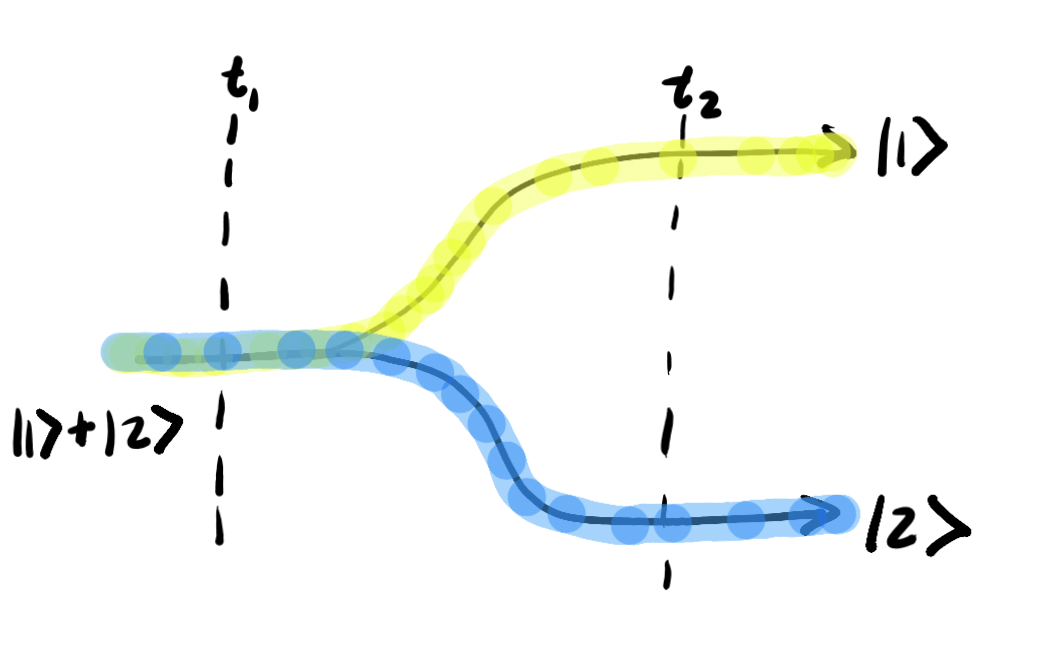
\includegraphics[width=0.7\textwidth]{lewis.png}
	\caption{Personal Identity and Branching Worlds}
	\label{f:lewis}
\end{figure}
At time $t_2$ after this two-state system has been measured, there are two sucessors, one on each branch. At time $t_1$, each of the branched persons overlaps. The agent on each branch is about to measure the system $\ket{1} + \ket{2}$, and since their situations are identical, they are unsure which person they are. 

This is not an argument so much as it is an explanation of subjective uncertainty. You could just as easily reject this view of personal identity in favor of option (3), so Wallace motivates (2) another way. The argument runs as follows \parencite[9-11]{wallaceLanguageUseBranching2005} :
\begin{enumerate}
	\item Imagine a similar universe to ours ($U^*$) whose physicists believe that their world does not branch. Philosophers believe that the correct tenseless semantics are linear (e.g. "it will rain tomorrow" = "it rains at time $s>t$" where $t$ is the time the statement is uttered). 
	\item Philosophers believe that branched semantics are incorrect (e.g. "it will rain tomorrow" is true on branches/histories where it does rain, and false where it doesn't, and since there is no matter of fact about which branch utterers are on, the statement is both true and false)
	\item Philosophers in $U^*$ determine that agents can rationally assign probabilities from 0 to 1 based on their credence in tenseless statements.
	\item However, physicists in $U^*$ are incorrect. $U^*$ is not linear, but a branching universe.
\end{enumerate}
There are two ways to make sense of this picture.
\begin{quote}
	\emph{Elite View}: The philosophers are right to apply linear semantics to the language of people within $U^*$. The consequence of this is that statements made in $U^*$ are almost always incorrect since the inhabitants are actually in a branching universe. Wallace demonstrates that ``there are no candidate ‘branch-talk’ sentences to express such truth-conditions without making most of our ‘ordinary’ future-directed sentences (like ‘it will rain tomorrow’) trivial or meaningless'' \parencite[9]{wallaceLanguageUseBranching2005}.
\end{quote}

\begin{quote}
	\emph{Charitable View}: The philosophers are wrong to apply linear semantics to the language of people within $U^*$. Applying branching-semantics makes true most of the statements made in $U^*$.
\end{quote}

On both views, the inhabitants of $U^*$ are incorrect in some regard. Wallace argues that the Charitable View is preferable if one takes the approach to semantics offered by Davidson, Lewis, and Quine (among others), specifically that if ``there are no further facts about meaning beyond fit to usage and the best interpretation is, other things being equal, that which makes most of the community’s utterances come out true'' \parencite[15]{wallaceEpistemologyQuantizedCircumstances2006}. Considering our own universe $U$ on the Charitable View, provided we really are in a branching universe, then we ought to consider talk of uncertainty as being correct / justified. Furthermore, if there really is uncertainty, then by restating the decision theoretic axioms \parencite{wallaceEverettianRationalityDefending2003a}, the weights given by the Born Rule just are the probabilities per the Principle Principle.
 \vspace{2em}
\todo[inline,caption={}]{TODO: Worries regarding Wallace's view:
	\begin{itemize}
		\item Is Quine's approach to semantics the right one to have? Are all things ``equal'' as they must be to prefer the Charitable View?
		\item Does this argument about the semantics of $U^*$ really track to our world $U$ in a way relevant for applying the Charitable View to our own semantics?
		\item Consider an alternative to the Elite View from Lewis' metaphysics (described by Wallace also). Is this the only path to uncertainty on Wallace's view?
	\end{itemize}}





\subsection{Fission (Greaves)}

Hilary Greaves is a vocal defender of the fission approach to understanding probability on the many worlds view \parencite{greavesEverettEvidence2010, greavesProbabilityEverettInterpretation2007, greavesUnderstandingDeutschsProbability2004}. 
Her view rejects subjective uncertainty—simply accepting (3) as a consequence of Everett's interpretation.
Rather than trying to make sense of uncertainty, she simply rejects that an agent could be uncertain in the case of branching.
Fissioners accept that an agent should rationally expect to see, with certainty, that each state in a given superposition will obtain. 
Yet, an agent can only experience seeing one state obtain, and so expectation is seemingly at odds with experience.

The fission program draws on decision theoretic axioms, similar to Wallace's view, in order to construct rational constraints on a branching agent. 
The decision theoretic axioms are proved in this branching context so as to connect an agent to their many branched successors \parencite[18]{wallaceEpistemologyQuantizedCircumstances2006}. 
A ``caring measure'' can then be constructed such that an agent places stock in each of their branched selves which will obtain after a quantum event. Each branched self is cared about with weight equal to the Born-rule amplitudes \parencite[sec. 3.1.2]{greavesProbabilityEverettInterpretation2007}. Before demonstrating Greaves' preferred argument for why the weights should be set to the Born-rule amplitudes, its worth considering a quick example of how an agent on the fission view makes sense of quantum outcomes.

What does this look like for an agent? Let’s take a simple example of a spin 1/2 system prepared in the laboratory with non-equal squared amplitude for each state of a particle:\footnote{Spin is an intrinsic angular momentum of particles. Like position and energy, quantum mechanics describes the ``likelihood'' of finding a particle in a particular spin state. In this case, the particle can have either spin-up or spin-down.}
\begin{gather}
	\ket{\Psi} = \frac{1}{\sqrt{5}}\left(2\ket{\uparrow} - \ket{\downarrow}\right)
\end{gather}
On the orthodox view, the probability of up is 4/5 and the probability of down is 1/5 as given by the square of the coefficient for each state.
A PI in the lab offers a wager to her research assistant. If the assistant observes the particle and finds spin up (down) then she will win (lose) \$20. Should the assistant take the bet? The assistant, having recently attended a lecture on many-worlds, knows that each state will necessarily obtain. At first, she is compelled to decline the bet because she knows she will lose \$20 no matter what (on one branch, at least). She then considers the set of branching futures which will occur if she takes the bet, and assigns a caring measure to each of her two branched selves (in this case, $4/5$ for up and $1/5$ for down). In this sense, she should care twice as much about the future on which she wins compared to the future in which she loses. With the odds in her favor, she takes the bet and branching occurs. The caring measure’s constraint on her rational preferences allows her to act as if she never went to the lecture at all and simply accepted the Born Rule probabilities. 

This picture is no doubt a confusing one. A rejection of uncertainty and probability (she sees no odds associated with winning and losing), an acceptance that all possible states occur (she will both win and lose), yet she prefers taking the bet over not (a consequence of the caring measure). The way I have set up the fission schema for understanding probability, or lack thereof, is missing one key connection. If the caring measure assigns weights to branches, \emph{why is it that those weights just are the squared amplitudes?} Can we provide a better connection between the physics and our reality than postulating that the weights just are the squared amplitudes as in the \emph{Born rule}?

\subsection{Measurement Neutrality and Equivalence}

The connection between square amplitudes and caring measures (or weights) is said to follow from two assumptions. These assumptions are said to be equivalent, and a proof is available from  \parencite[10]{greavesProbabilityEverettInterpretation2007}:

\begin{quote}
	``Measurement Neutrality:  A rational agent is indifferent between any two quantum bets that agree on the state $\ket{\psi}$  on which the measurement is to be performed, the observable $\hat{X}$ to be measured, and the  `payoff function' $P$ from the spectrum of $\hat{X}$ to the set of consequences.''
\end{quote}

\begin{quote}
	``Equivalence:  A rational agent is indifferent between any two quantum bets that agree, for each possible reward, on the mod-squared measure of branches on which that reward is given.''
\end{quote}

\emph{Measurement Neutrality} (MN) on its face is highly plausible. If two bets or wagers agree on the state and the measurement, and their payoff functions spit out the same rewards or consequences, then an agent should not prefer one over the other. It is not immediately obvious how \emph{Equivalence} (EQ) is itself equivalent to MN, but as Greaves notes, a proof is available in Wallace (\citeyear{wallaceQuantumProbabilitySubjective2005} p. 12-14).\footnote{Wallace argues that MN lacks force outside the Subjective Uncertainty viewpoint (in \textsection \ref{SU}) because a measurement is an ``unnatural category'' and the manner in which measurements processes track to decision theoretic measurement-talk is incoherent \parencite{wallaceEpistemologyQuantizedCircumstances2006}. Fissioners like Greaves need not worry, as Wallace provides two direct justifications for EQ. }

Accepting these assumptions, we can now consider Greaves' justification for recovering the Born-rule amplitudes on the fission view. She does so by considering weighting functions which satisfy the branching decision theoretic axioms but violate EQ. The first rule one might consider for rational branch assignments is to allow any function for determining the weights:
\begin{quote}
	``Full permissivism: Any probability measure on the set of possible branches is rational''\parencite[11]{greavesProbabilityEverettInterpretation2007}.
\end{quote}
Greaves then draws up some potential functions, one where an agent assigns weights to branches based on the number of socks one possesses after a measurement pre-branching, another where the actual value of the observable (for example, the position of a measured particle by some metric/unit) is used to determine the weight. While these methods are bizarre, it is entirely rational under full permissivism and consistent with MN/EQ. There are, however, particular measures which can be discarded. One such method of probability assignment discarded by Greaves is \emph{Naïve Counting}.
\begin{quote}
	``Naive Counting: All branches are to be assigned equal measure''\parencite[11]{greavesProbabilityEverettInterpretation2007}.
\end{quote}
She claims that this method fails under decoherence because there is inherent vagueness in the way one carves up the branching structure. 
This objection is similar to the preferred basis problem, wherein a particular basis (for example, energy) will produce a wholly different branching structure from another basis (for example, spin), and so the task of carving probability space into a set of concrete histories is unclear.
Her claim is that the branching structure is vague even if one can defend that a particular basis is special in some way. 

Her argument against full permissivism is an interesting one.
\begin{quote}
 ``Given that the actual physical state of the universe is the physical state, the measure given by using the mod-squared prediction in conjunction with that state is overwhelmingly more natural than the measure given by Relevance of Socks (why socks, rather than pants?), or any of the arbitrarily complicated measures allowed by full permissivism'' \parencite{greavesProbabilityEverettInterpretation2007}.
\end{quote}
The claim here is that the naturalness of the function for assigning weights to branches is an important feature, one which makes the Born-rule function more rational than others. Even though there are other permissible functions for assigning weights, since the Born-rule is the most natural, it is therefore more sensible to adopt that one.

 \vspace{2em}
\todo[inline,caption={}]{TODO: Worries regarding Greaves' view:
	\begin{itemize}
		\item Why does naturalness govern the rationality of assigning weights to branches? 
		\item Why is it that only Naïve Counting is susceptible to the objection regarding vagueness in precisifying branches / decoherence?
		\item Consider an alternative view from Jake Khawaja on branch counting and weighting of branches.
\end{itemize}}

\subsection{References}
\printbibliography[heading=none]

\section{Methods}

\emph{How are you conducting your research?
What procedures or techniques are you using to gather information/data for your thesis?
What resources or materials are you using in your research?
Describe any specialized training you have received or will receive to conduct your research (e.g., lab safety certification or human/animal testing, training to conduct interviews or focus groups), and indicate who provided the training.
}

\vspace{2em}
\noindent Research is conducted by reading existing philosophical literature on many-worlds and probability. Materials and training N/A.

\section{Evaluation}
\emph{How will your work be reviewed and graded?
What measurable goals does your research committee expect you to accomplish during the final stages of your Research Manuscript/Creative Portfolio?
How will your committee provide feedback regarding your progress?
How will your committee assess the viability of your research to produce a Research Manuscript/Creative Portfolio with a final presentation of your work?
If you are registering for a CreativePortfolio, be specific about the artifact that you will produce in addition to the written component/reflection (e.g., a novel, poetry collection, art DVD, case study, engineering design, story board, film DVD, or musical composition CD or DVD).
}

\vspace{2em}
\noindent
The manuscript is to be assessed on the strength of the claims made, accuracy and coherence of reconstructed arguments, and relevance of the worries and counter-arguments raised throughout.
Feedback on the manuscript to be relayed informally during meetings between committee members and myself or through formal comments on the working document.  

\section{Communication}
\emph{
What are the expectations about meetings with your faculty sponsor and other committee member(s)? Be specific.
How often are you meeting with your faculty sponsor? How often will you meet with the full committee? A general guideline is to meet with your faculty sponsor 30 min/week or 60 min/every other week to maintain communication, assess progress, troubleshoot problems, etc.
What are your faculty sponsor's expectations of such meetings? What are your committee members’ expectations about meeting with you?
What time commitment (number of hours of work per week) is expected to be applied to your research between meetings with your faculty sponsor?
}

\vspace{2em}
\noindent
The expectation is to continue raising questions with focus narrowed towards the views described in \textsection 2 during 60min/every other week meetings with faculty sponsor. Particularly, the focus of meetings in the 499T/P semester will be geared towards clarifying objections and worries against these prominent views, constructing alternative views/arguments where applicable, and ultimately weighing the virtues of adopting one stance over the other (subjective uncertainty v.s. fission). Above all, the goal of meetings is to address issues/concerns with the drafting of the final manuscript.

\section{Timeline}
\emph{
What are the dates and expectations for periodic review of your research results? (weekly? bi-weekly?)
What are the due dates for your manuscript:
Outline?
First draft?
Second draft?
Final written component?
Artifacts (for Creative Portfolios)?
What is the date and setting for the final presentation of your work (e.g., informal with 499T/P committee members only or public presentation open to others)?
}

\vspace{2em}
\noindent
Version control with change log of manuscript maintained with Git repository, therefore review of changes can be performed at every other meeting.

\vspace{2em}
\noindent
Draft: due March 31st.\\
Final: due April 30th.\\
Presentation: TBD, private, informal with committee.

\end{document}
